\documentclass[border=3pt]{standalone}
% Preâmbulo compartilhado pelos diagramas TikZ da aula 5 de IHC (Processos de Design)
\usepackage[T1]{fontenc}
\usepackage[utf8]{inputenc}
\usepackage{lmodern}
\usepackage{amsmath}
\usepackage{xcolor}
\usepackage{tikz}
\usetikzlibrary{arrows.meta,angles,quotes,decorations.pathmorphing,calc,
                positioning,shapes.geometric,shapes.misc,backgrounds,fit,
                math}

% Paleta (mesma dos SVGs originais)
% Paleta da disciplina de IHC: acento roxo (#755099), da capa do livro.
% (o nome "dblue" é mantido para não alterar todos os diagramas)
\definecolor{dblue}{HTML}{755099}
\definecolor{dorange}{HTML}{B3541E}
\definecolor{dgreen}{HTML}{4A7C59}
\definecolor{dred}{HTML}{9C4B4B}
\definecolor{dcream}{HTML}{F4F1EA}
\definecolor{dshade}{HTML}{DDD7C9}

% Função gaussiana (não normalizada por padrão de escala visual)
\pgfmathdeclarefunction{gauss}{3}{%
  \pgfmathparse{1/(#3*sqrt(2*pi))*exp(-((#1-#2)^2)/(2*#3^2))}%
}

% Estilos comuns (prefixo d... para não colidir com chaves internas do pgf)
\tikzset{
  >={Stealth[length=2mm]},
  dguide/.style={gray!55, dashed, line width=0.4pt},
  daxis/.style={gray!60, line width=0.7pt, ->},
  dbody/.style={fill=black!3, draw=black!80, line width=1pt},
  dacc/.style={draw=dblue, line width=1pt},
  dlbl/.style={black!55, font=\small},
  dsub/.style={black!45, font=\footnotesize},
  dstate/.style={circle, draw=black!80, fill=dcream, line width=1pt,
                 minimum size=17mm, font=\large, inner sep=1pt},
  dobs/.style={circle, draw=black!80, fill=dshade, line width=1pt,
               minimum size=14mm, font=\large, inner sep=1pt},
  dbox/.style={rounded corners=2pt, draw=black!80, fill=dcream, line width=1pt,
               align=center, inner sep=6pt},
  dop/.style={circle, draw=black!80, fill=white, line width=1pt,
              minimum size=6mm, inner sep=0pt, font=\small},
  dtrans/.style={->, dblue, line width=1pt},
  dmeas/.style={->, dorange, line width=1pt},
  dcurve/.style={line width=1pt, dblue},
  dcurveb/.style={line width=1.4pt, dorange},
}

\begin{document}
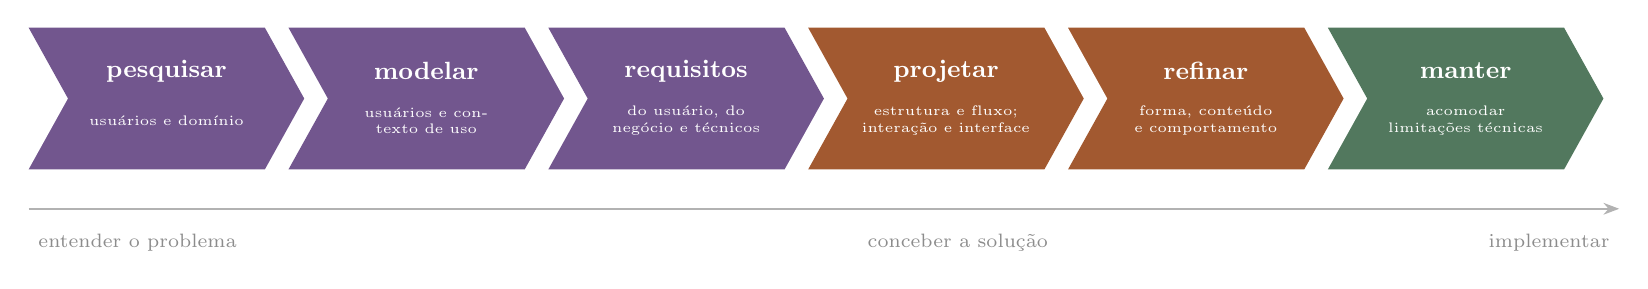
\begin{tikzpicture}[x=1cm,y=1cm]

  \newcommand{\chev}[4]{% x  titulo  subtitulo  cor
    \fill[#4!85!black, opacity=0.9] (#1,0) -- (#1+3.0,0) -- (#1+3.5,0.9) -- (#1+3.0,1.8) -- (#1,1.8) -- (#1+0.5,0.9) -- cycle;
    \node[white, font=\bfseries\small] at (#1+1.75,1.25) {#2};
    \node[white, font=\tiny, text width=2.3cm, align=center] at (#1+1.75,0.62) {#3};}

  \chev{0}{pesquisar}{usuários e domínio}{dblue}
  \chev{3.3}{modelar}{usuários e contexto de uso}{dblue}
  \chev{6.6}{requisitos}{do usuário, do negócio e técnicos}{dblue}
  \chev{9.9}{projetar}{estrutura e fluxo; interação e interface}{dorange}
  \chev{13.2}{refinar}{forma, conteúdo e comportamento}{dorange}
  \chev{16.5}{manter}{acomodar limitações técnicas}{dgreen}

  \draw[daxis] (0,-0.5) -- (20.2,-0.5);
  \node[dsub, font=\scriptsize, anchor=north west] at (0,-0.7) {entender o problema};
  \node[dsub, font=\scriptsize, anchor=north] at (11.8,-0.7) {conceber a solução};
  \node[dsub, font=\scriptsize, anchor=north east] at (20.2,-0.7) {implementar};


\end{tikzpicture}
\end{document}
